\section{Evaluation on Aggregate Human Occupancy Behaviour Dataset}
\label{sec:evareal}

Having evaluated the performance of POPP and FOPP filters on simulated data, we now move to evaluate the performance of all POPP models on a large, real-world data set with the FOPP model as the base model.

\begin{figure}[t]
	\centering
    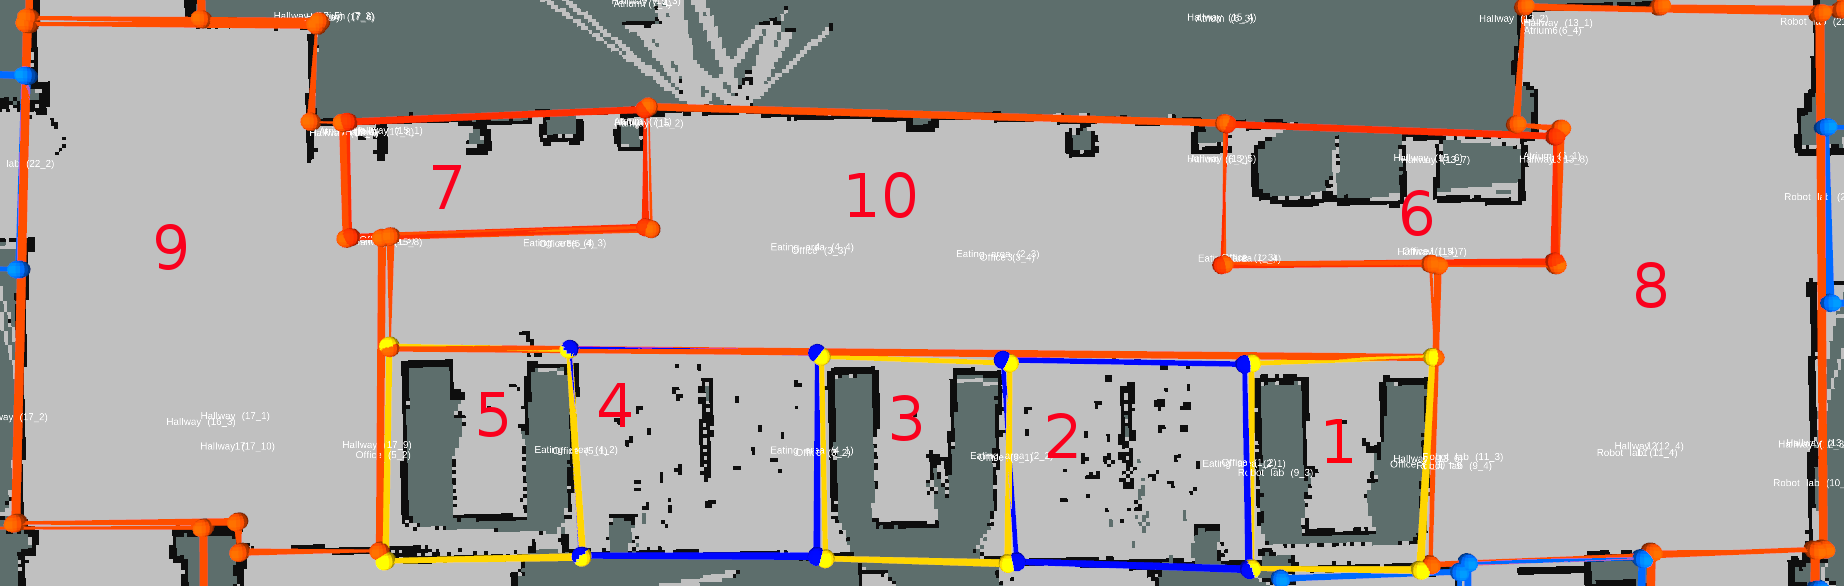
\includegraphics[width=0.5\textwidth]{./figures/map_popp.png}
    \caption{The office building in which the robot gathered data. Areas are bounded by imaginary lines.}
    \label{fig:map_popp_independent_test}
\end{figure}

This dataset is a collection of counts over time from three different automated person detectors. These use laser (leg detector - LD), depth camera (upper body detector - UBD), and RGB information (change detector - CD). The dataset was gathered from an office building where a mobile robot counts and observes the number of people passing by as it patrols around the area (see Figure~\ref{fig:map_popp_independent_test}). Each detector/sensor returns a sensed count of the number of people it detected in each 10 minute interval during the day. These detectors are unreliable and some examples of (true and false) positive and (true and false) negative detections made by the detectors can be seen in Figure~\ref{fig:sensor_images}.

\begin{figure}[t]
	\centering
	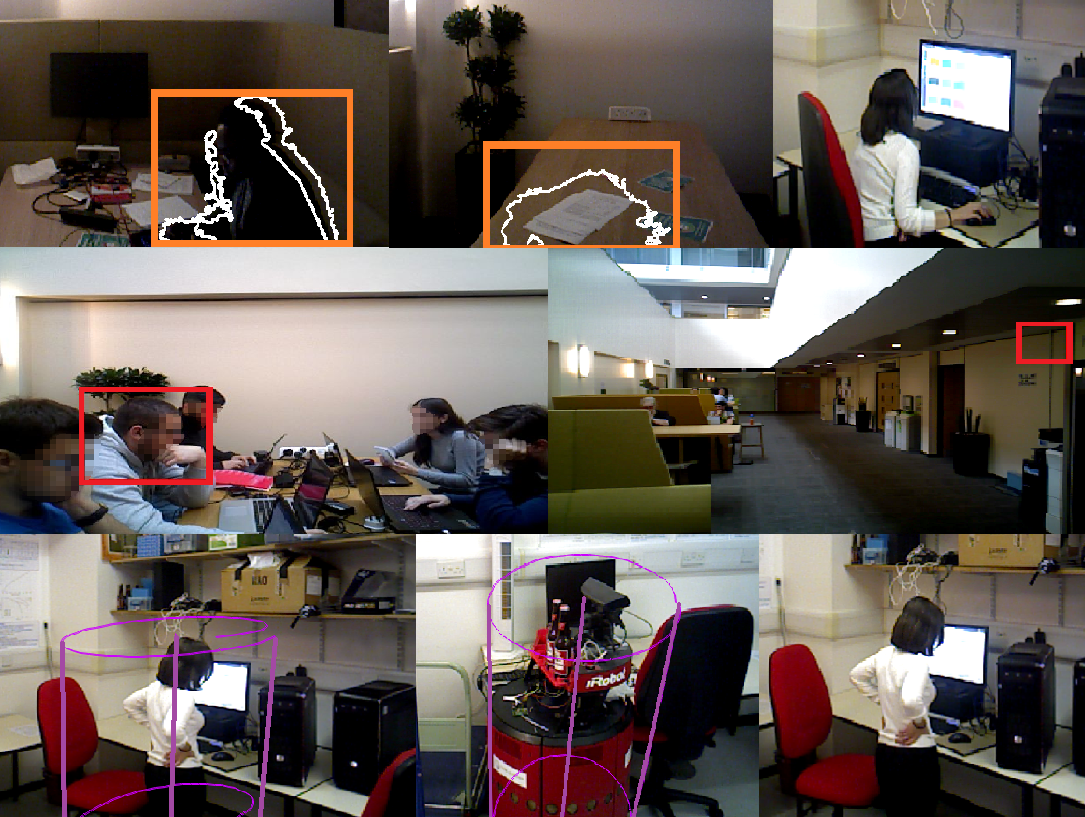
\includegraphics[width=0.5\textwidth]{./figures/sensor_images.png}
	\caption{True/False positive detections and true/false negative detections from different areas for each detector. Top row: change detector. Middle row: upper body detector. Bottom row: leg detector. Detections are marked with 2D or 3D bounding boxes.}
    \label{fig:sensor_images}
\end{figure}

The data set was gathered during a deployment of the mobile robot at the lower ground of the computer science building in University of Birmingham. As a mobile robot can not fully sense its environment, it can only perceive partial data at a particular time and place. Moreover, the robot's patrol policy also affects where and when detections are perceived. Consequently, the detections are temporally and spatially scattered and they are not uniformly distributed across space. The detections are then organised according to time/date and the spatial region where each detection was made.

During the deployment of the mobile robot, ground truth data were also gathered to create sensor unreliability models, one for each detector in each area. Both the joint sensor model and the standard sensor model must be trained from sensor counts and true counts. The sensor models were built from the data collected from 10am-8pm each for 48 days. A four fold cross-validation on the 48-day dataset with the unit being a whole day was carried out, where 12 days of data were used to train the sensor model. This process is done for all areas within the patrol space.

The true $\lambda$ for the Poisson process and $\lambda(t_i, t_j)$ for the periodic Poisson process on each region was estimated by running a FOPP filter on the true counts. The uncorrected estimate $\lambda$ according to the FOPP model was estimated only from the change detector count data since the change detector is the most reliable detector among three detectors available. Using RMSE and the Jensen-Shannon distance, the estimated true $\lambda$ and its distribution are then used as a comparison to the resulting estimated $\lambda$ (and $\lambda(t_i, t_j)$ respectively) produced by each filter.

\begin{figure}[t!]
	\centering
	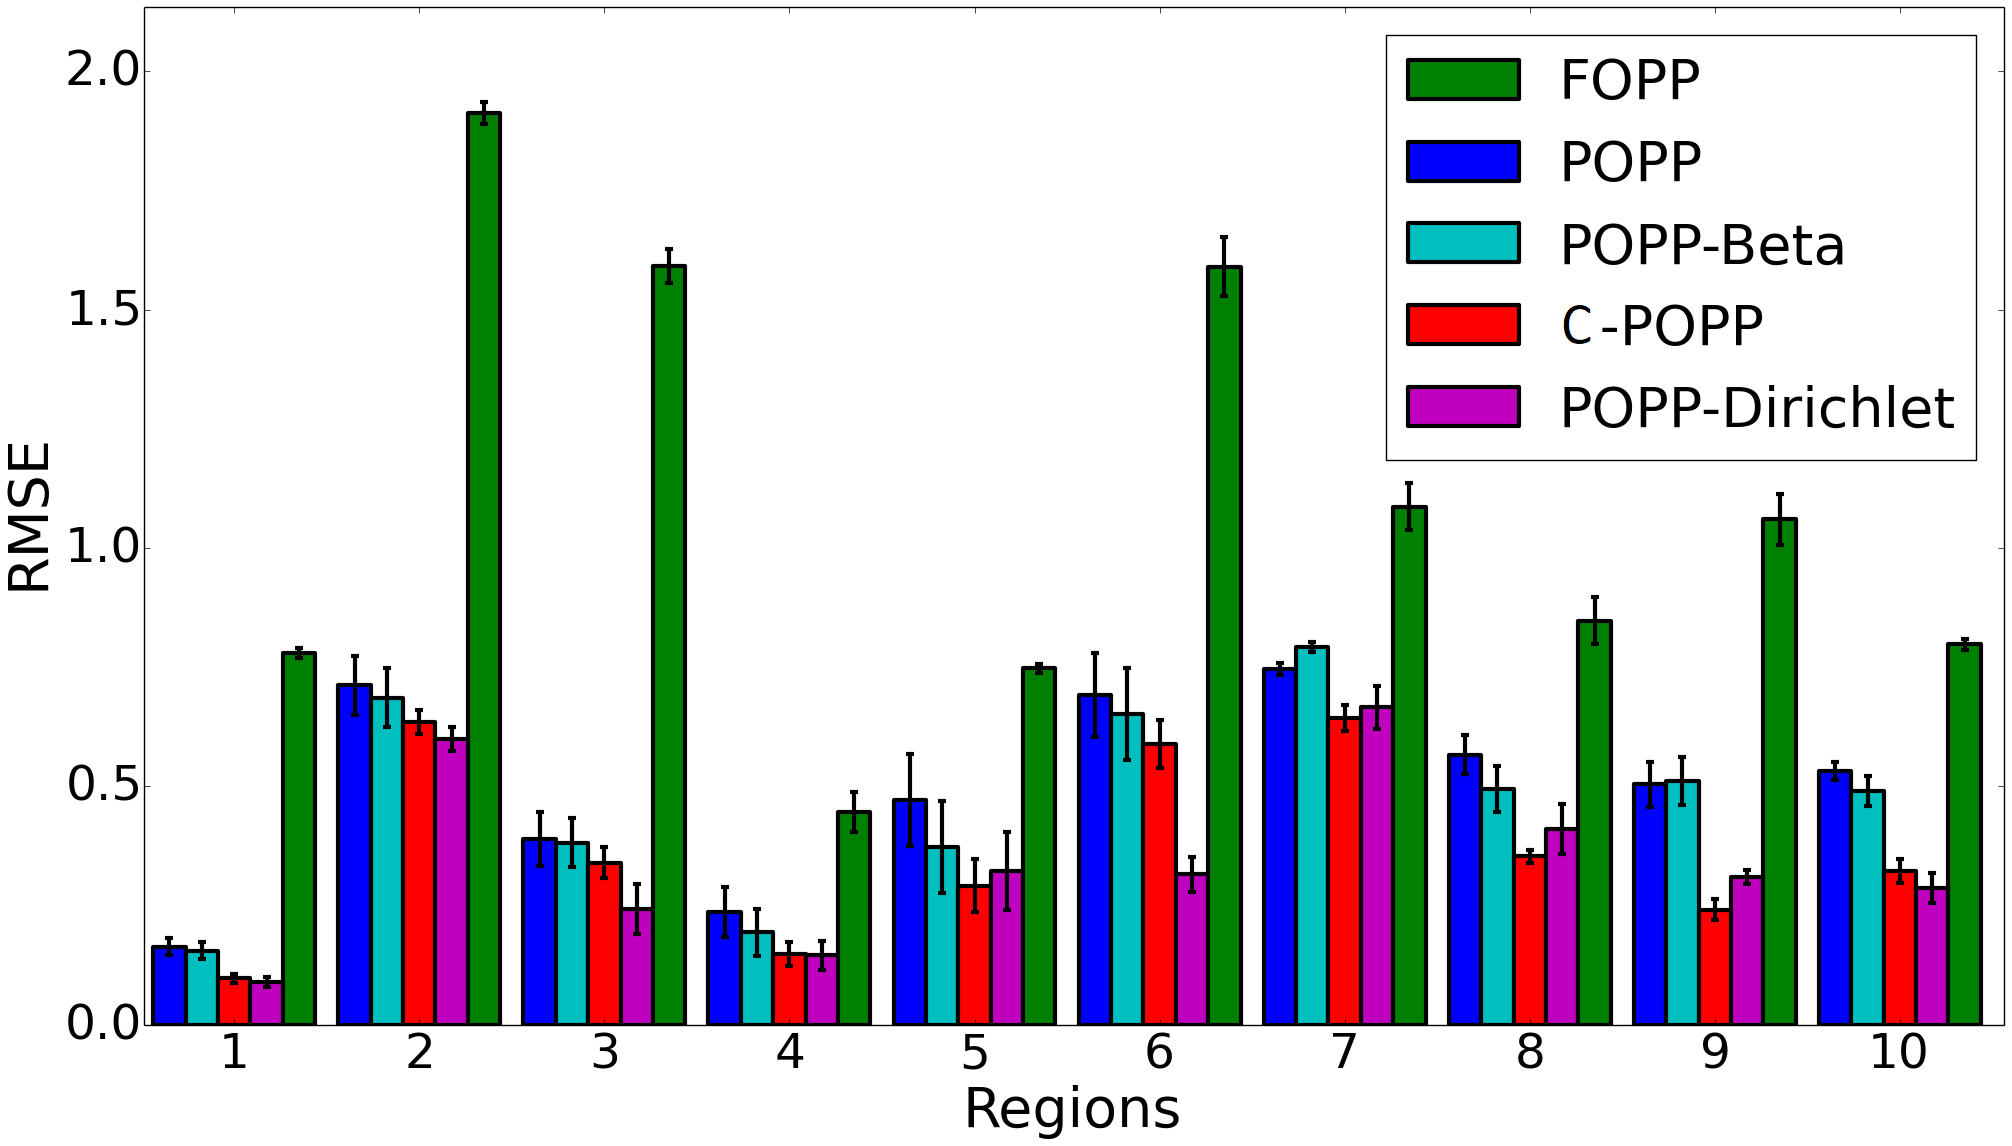
\includegraphics[width=0.5\textwidth]{./figures/rmse_across_region_popp_dirichlet.png}
    \caption{The RMSE of the FOPP, POPP, POPP-Beta, and POPP-Dirichlet estimators of $\lambda$ as it varies across areas (regions) of the environment. Standard error is shown.}
    \label{fig:rmse_across_region_popp_dirichlet}
\end{figure}

\begin{figure}[t!]
	\centering
	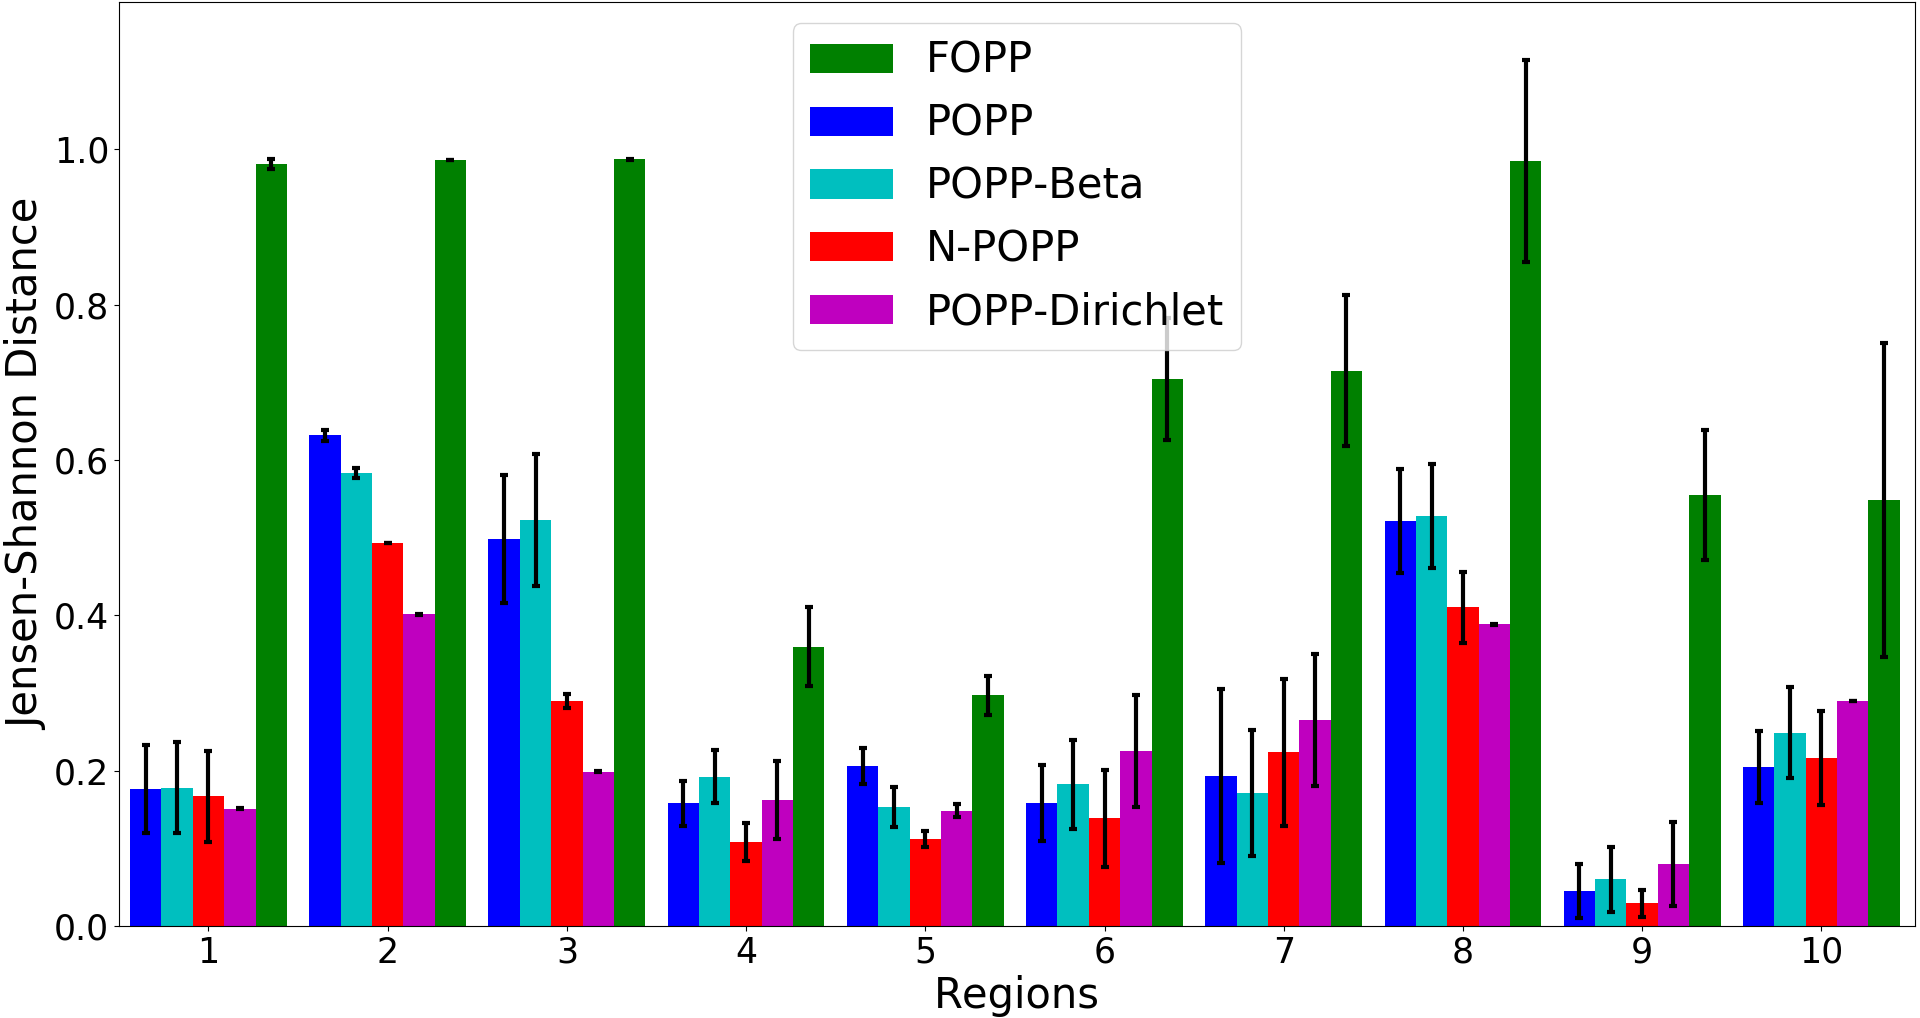
\includegraphics[width=0.5\textwidth]{./figures/fopp_popp_popb_npop_popd_homo_kl.png}
	\caption{The Jensen-Shannon distance of the FOPP, the POPP, the POPP-Beta, the N-POPP, and the POPP-Dirichlet model distributions of $\lambda$ as it varies across areas (regions) of the environment. Standard error is shown.}
	\label{fig:fopp_popp_popb_npop_popd_homo_kl}
\end{figure}

\begin{figure}[t!]
	\centering
	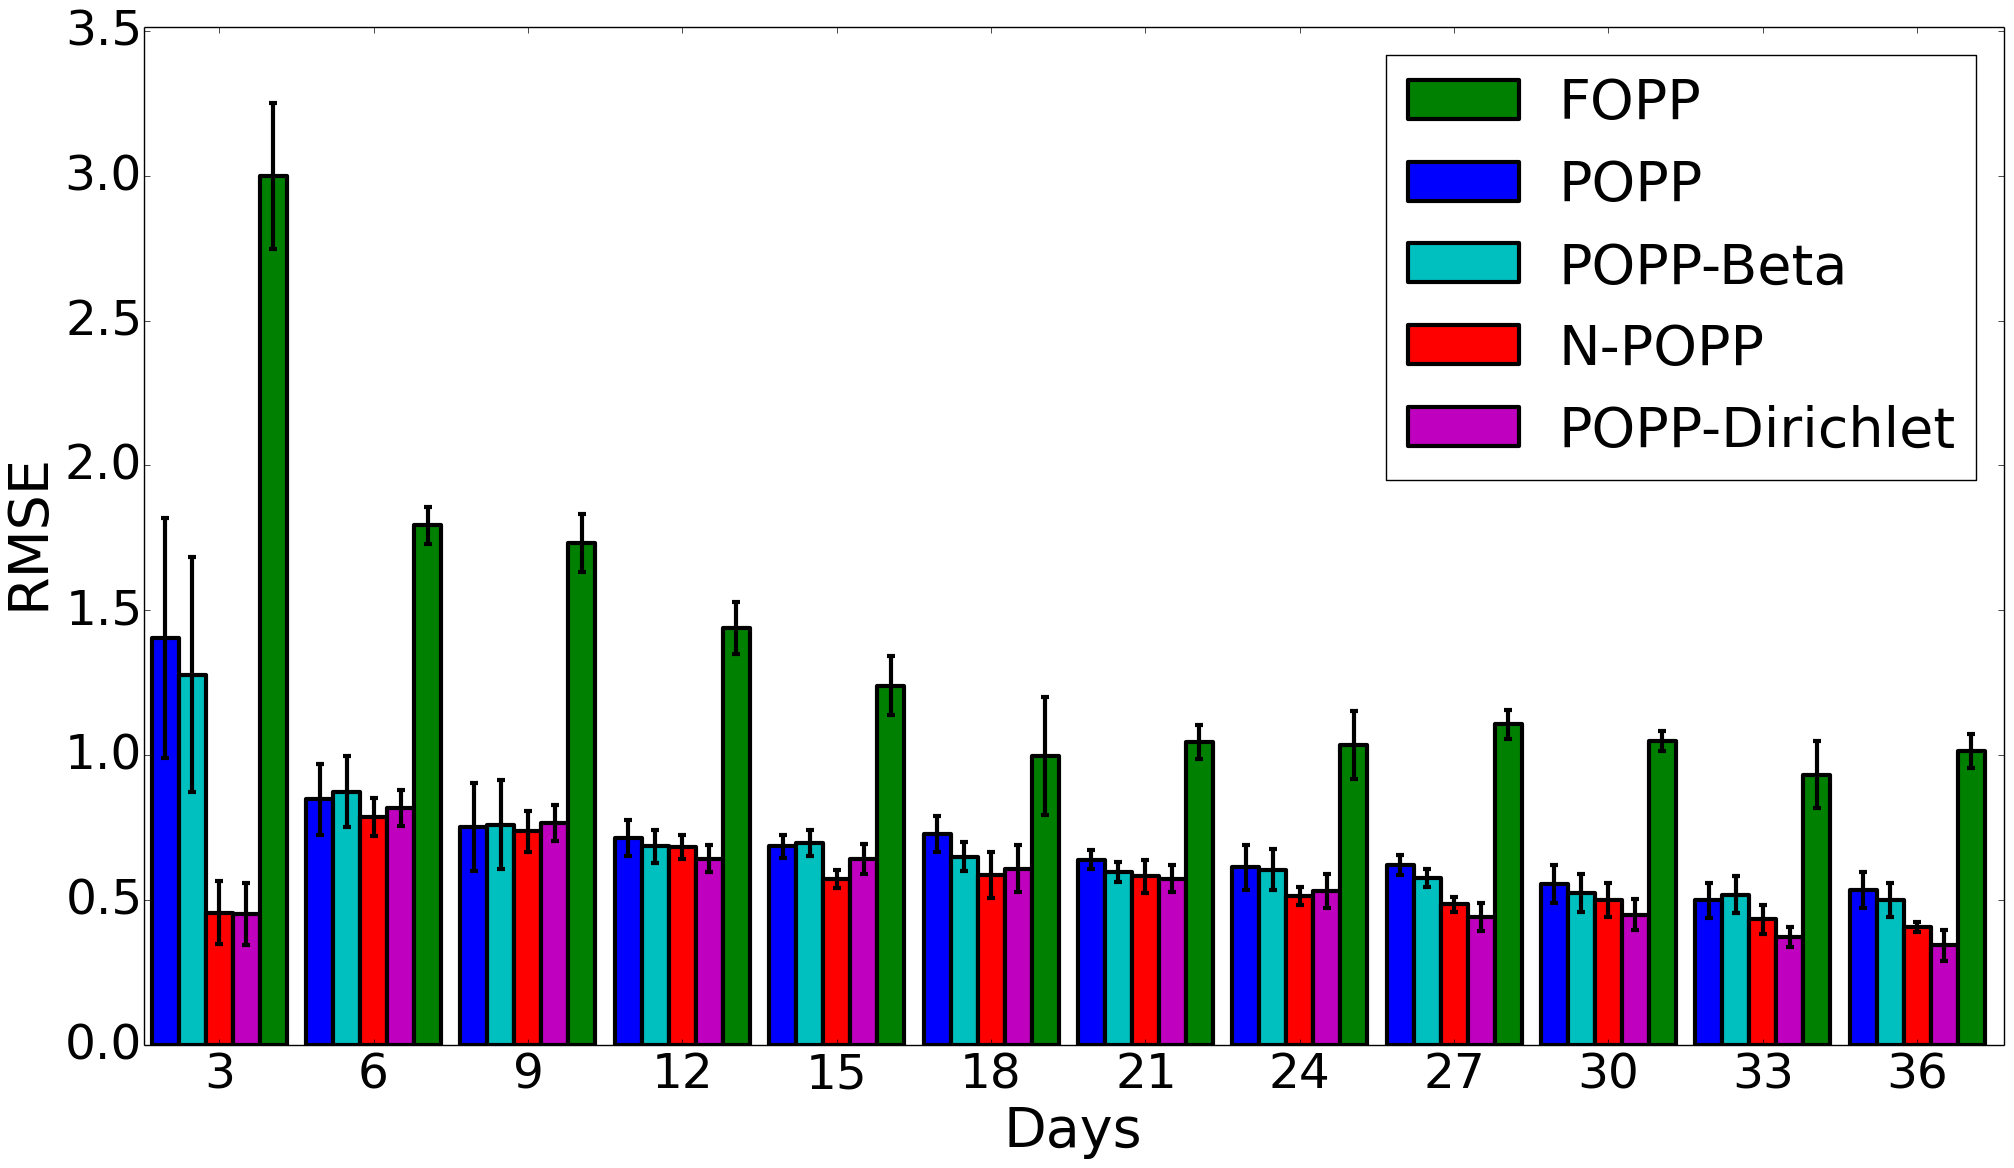
\includegraphics[width=0.5\textwidth]{./figures/rmse_evolution_popp_dirichlet.png}
	\caption{The RMSE evolution from day 3 to day 36 with 3 day interval, averaged across all regions. Standard error is shown.}
	\label{fig:rmse_evolution_popp_dirichlet}
\end{figure}

\begin{figure}[t!]
	\centering
	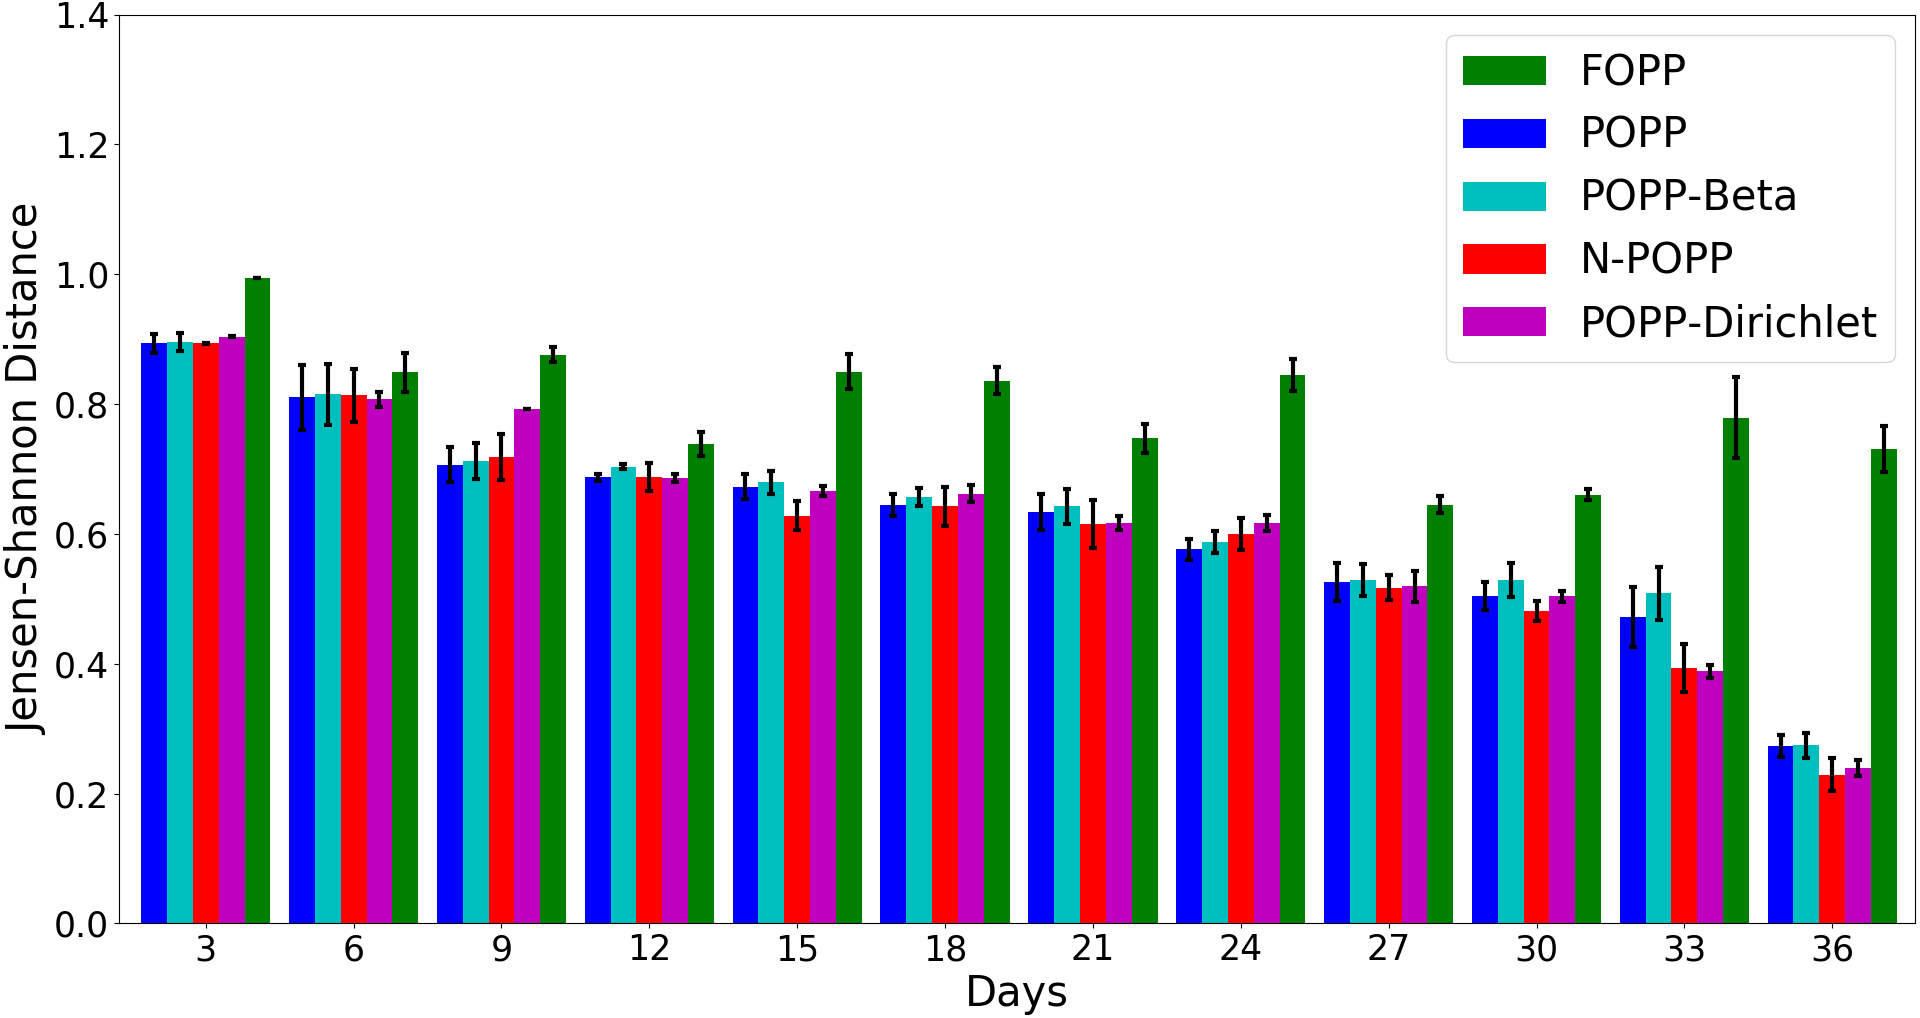
\includegraphics[width=0.5\textwidth]{./figures/fopp_popp_popb_npop_popd_homo_kl_evo.png}
	\caption{The Jensen-Shannon distance evolution of the FOPP, the POPP, the POPP-Beta, the N-POPP, and the POPP-Dirichlet model distributions of $\lambda$ from day 3 to day 36 with 3 day interval, averaged across all regions. Standard error is shown.}
	\label{fig:fopp_popp_popb_npop_popd_homo_kl_evo}
\end{figure}
